\documentclass[11pt, letterpaper]{article}

% --- PREÁMBULO (Configuración) ---
\usepackage[utf8]{inputenc} % Permite usar tildes y eñes directamente
\usepackage[spanish]{babel} % Traduce elementos automáticos (ej. "Date" a "Fecha")
\usepackage{amsmath}        % Herramientas matemáticas avanzadas
\usepackage{authblk}        % para poner la universidad
\usepackage{booktabs}
\usepackage{float}
\usepackage{tabularx}
\usepackage[font=small,labelfont=bf,textfont=it]{caption}
\usepackage{graphicx}
\usepackage{siunitx}
\usepackage{makecell}
\usepackage{array}
\usepackage{amssymb}

\title{
    \rule{\linewidth}{0.4mm} \\[0.4cm] % Línea superior
    \huge \textbf{Construcción y análisis de una función hash artesanal} \\[0.2cm]
    \Large \textit{ Universidad Anáhuac - Blockchain} \\[0.1cm]
    \rule{\linewidth}{0.4mm} % Línea inferior
}
\author{
    \textbf{Santiago Cosme Cervera} \\
}
\date{\today}

% --- CUERPO DEL DOCUMENTO ---
\begin{document}

\maketitle % Imprime el título usando los datos del preámbulo

\begin{abstract}
    Una función hash utilizada para aplicaciones reales garantiza 
    su seguridad al cumplir con cuatro propiedades de seguridad: 
    efecto avalancha, resistencia a colisiones, resistencia a preimagen y resistencia a segunda preimagen.
    Esta tarea propone una función hash artesanal y busca comprender de manera cuantitativa
    las propiedades de seguridad fundamentales a través de pruebas. No busco construir una función
    hash segura, si no que busco medir con rigor por qué no lo es. 
\end{abstract}

\section{Diseño}
\subsection{Definición formal de la función hash}
La función hash propuesta se define de la siguiente manera
\begin{equation}
    H : \{0, 1\}^* \rightarrow \{0, 1\}^{32}
\end{equation}
donde cada mensaje \textit{m} se convierte en una secuencia binaria y se procesa en bloques de 32 bits. La salida
tiene una longitud fija de 32 bits, lo cuál equivale a 8 dígitos hexadecimales.\\

Para convertir el mensaje original \textit{m} a binario, primero obtenemos la codificación ASCII de cada carácter (cada símbolo se convierte en 8 bits).
Así, si $m = c_1 c_2 \dots c_k$, entonces:
\begin{equation}
    B(m) = bin(ASCII(c_1)) || bin(ASCII(c_2)) || \dots || bin(ASCII(c_k))
\end{equation}

\subsection{Esquema de padding}
Para asegurarse de que el mensaje quede dividido en bloques de 32 bits, se debe de aplicar un esquema de \textit{padding}.
Lo defino de la siguiente manera:
\begin{equation}
    P(B) = B || 1 || O^k || len(B)_{32}
\end{equation}
donde 1 es un bit de marca, $0^k$ representa una secuencia de ceros y $len(B)_{32}$ la longitud original del mensaje. El valor de \textit{k} se selecciona de manera que la longitud resultante sea múltiplo de 32. 
\subsection{Estado interno}
El algoritmo mantiene un estado interno de 32 bits. Se inicializa con la constantes:
\begin{equation}
    h_0 = 01101010000010011110011001100111
\end{equation}
equivalente al valor hexadecimal \textit{0x6a09e667}. Este valor son los primeros 32 bits de la parte fraccionaria de $\sqrt{2}$ y sirve como el punto de partida para la actualización iterativa del digest.\\

Sea $P(B) = b_1 || b_2 || \dots || b_n$ con $|b_i| = 32$ para cada bloque $b_i$. El estado se actualiza en cada iteración mediante una función de compresión que toma como entrada el estado previo $h_{i-1}$ y el bloque actual $b_i$.
\subsection{Función de compresión}
La función de compresión se define como una mezcla de tres operaciones (rotación circular hacia la izquierda que aporta asimetría, suma modular que aporta difusión y XOR que aporta no linealidad) sobre palabras de 32 bits. Para cada bloque $b_i$, el algoritmo lo convierte en un entero y ejecuta 8 rondas de mezcla (este párametro puede cambiar). En cada ronda se aplica:
\begin{equation}
    t_{j+1} = ROTL_3((h_{i-1} + t_j + j)\; mod\; 2^{32} \oplus 0x55555555)
\end{equation} \newpage

donde:
\begin{itemize}
    \item $t_j$ es el valor intermedio en la ronda \textit{j}
    \item $j$ es el índice de la ronda
    \item $\oplus$ representa la operación XOR
    \item $ROTL_3$ denota una rotación circular hacia la izquierda de 3 posiciones
    \item 0x55555555 es una constante fija de 32 bits
\end{itemize}

Después de completar las rondas, el nuevo estado se actualiza mediante 
\begin{equation}
    h_i = (h_{i-1}+t_8) \; mod \; 2^{32}
\end{equation}

Finalmente, la salida del hash se obtiene como:
\begin{equation}
    H(m) = hex(h_n)
\end{equation}

\section{Método}
Para evaluar experimentalmente la calidad de la función hash, se analizaron cuatro propiedades fundamentales: efecto avalancha, resistencia a colisiones, resistencia a preimágenes y resistencia a segunda preimagen. En todos los casos se compara el valor experimental con su valor teórico esperado.

\subsection{Efecto avalancha}
Experimentalmente, se tomó un mensaje original y se alteró un único bit de su representación binaria. Luego se calculó el hash del mensaje original $H(m)$ y del nuevo mensaje alterado $H(m')$ y se midió la distancia de Hamming definida de la siguiente manera:
\begin{equation}
    d_H = \sum_{i=1}^{32}[H_i(m) \neq H_i(m')]
\end{equation}
El cálculo se repite para todos los bits del mensaje, y se calculó el promedio de bits alterados en la salida. En una función ideal, $E[d_H] = 16$ bits sobre 32, o un 50\% de los bits cambiados.
\subsection{Colisiones}
Experimentalmente, se truncó el digest a longitudes de salida de $d \in \{3, 4, 5, 6, 7\}$ dígitos hexadecimales. Para cada valor $d$, se generaron mensajes aleatorios y se calculó su digest truncado hasta encontrar dos mensajes distintos con el mismo valor. El número de intentos necesario para encontrar una colisión se registró y promedió sobre multiples ejecuciones.\\
El valor teórico esperado se aproxima mediante la "ley de cumpleaños":
\begin{equation}
    E[intentos] \approx \sqrt{\frac{\pi}{2}} \cdot 2^{2d}
\end{equation}
ya que el espacio de salida tiene tamaño $2^{4d}$ bits.
\subsection{Resistencia a preimágen}
Experimentalmente, se fijó un objetivo como un digest truncado $d \in \{3, 4, 5, 6, 7\}$ de longitud $d$, generado a partir de un mensaje previamente definido. Después se generaron mensajes aleatorios y se calculó su digest truncado hasta encontrar uno que coincidiera con el mensaje objetivo. La complejidad teórica esperada es
\begin{equation}
    E[intentos] = 2^{4d}
\end{equation}
dado el espacio de salida. Se requiere explorar aproximadamente la mitad del espacio antes de encontrar una preimagen.
\subsection{Resistencia a segunda preimágen}
Experimentalmente, se eligió un mensaje base $m$ y se calculó su digest truncado. Luego, se generaron mensajes distintos de $m$ y se buscaron coincidencias con el mimso digest objetivo. La expectativa teórica es la misma que para la preimagen:
\begin{equation}
    E[intentos] = 2^{4d}
\end{equation}

\section{Resultados}
A continuación se muestran los resultados de las pruebas de seguridad.
\subsection{Prueba 1: Efecto avalancha}

\begin{table}[H]
\centering
\small
\renewcommand{\arraystretch}{1.2}
\begin{tabularx}{\textwidth}{lXXXXXX}
\toprule
Mensaje & Long. & Intentos & $\bar{\delta}$ (bits) & \% cambio & $\sigma$ & [mín, máx] \\
\midrule
$a$ & 8 b & 8 & 15.38 & 48.05 & 1.77 & [13, 18] \\
$1$ & 8 b & 8 & 15.00 & 46.88 & 3.25 & [10, 19] \\
$ok$ & 16 b & 16 & 16.75 & 52.34 & 2.89 & [13, 23] \\
$no$ & 16 b & 16 & 17.56 & 54.88 & 2.73 & [14, 22] \\
$sol$ & 24 b & 24 & 16.33 & 51.04 & 2.99 & [9, 22] \\
$hola\ mundo$ & 80 b & 80 & 16.38 & 51.17 & 3.12 & [9, 22] \\
$criptografia$ & 96 b & 96 & 15.94 & 49.80 & 3.02 & [9, 24] \\
$universidad\ anahuac$ & 152 b & 152 & 15.99 & 49.98 & 3.13 & [7, 24] \\
$laboratorio\ blockchain$ & 176 b & 176 & 16.23 & 50.71 & 2.58 & [7, 21] \\
$tarea\ artesanal$ & 120 b & 120 & 16.00 & 50.00 & 2.57 & [10, 22] \\
\vdots & \vdots & \vdots & \vdots & \vdots & \vdots & \vdots \\
\midrule
Global & -- & 4416 & 15.97 & 49.90 & 2.84 & [7, 25] \\
\bottomrule
\end{tabularx}
\caption{Efecto avalancha observado para distintos mensajes. La métrica $\bar{\delta}$ representa la media de bits cambiados en la salida al alterar un solo bit de la entrada.}
\end{table}

La función hash cumple con una buena difusión al obtener un valor global de 49.9\% de bits modificados, muy cercano del valor ideal de 50\% que deben de tener las funciones hash.
\begin{figure}[H]
    \centering
    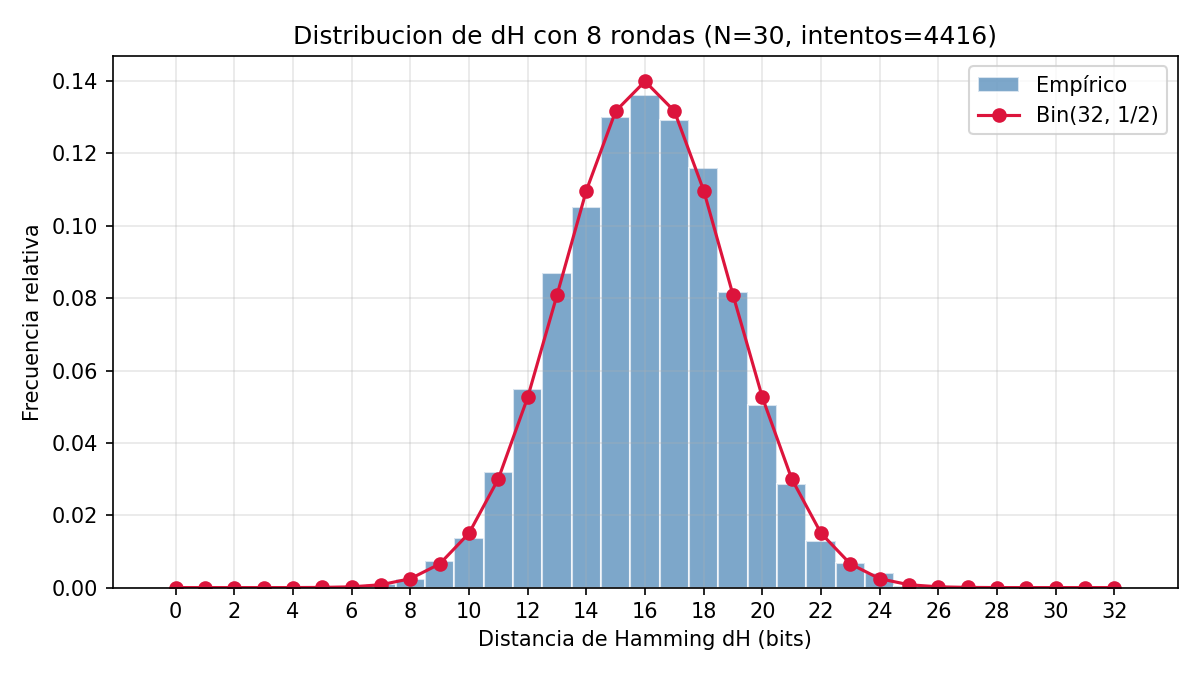
\includegraphics[width=0.9\linewidth]{../outputs/avalancha/avalancha_histograma.png}
    \caption{Efecto avalancha observado al variar el número de rondas del algoritmo.}
\end{figure}
Podemos observar en la \textit{Figura 1} cómo la distribución exeprimental cumple $X \sim Binomial(32, 0{.}5)$
\subsection{Prueba 2: Colisiones}
\begin{table}[H]
\centering
\small
\renewcommand{\arraystretch}{1.2}
\begin{tabularx}{\textwidth}{lXXXXXXX}
\toprule
$d$ (hex) & $n$ (bits) & Intentos teóricos & Intentos obs. & Tiempo medio (ms) & \makecell{Repeti-\\ciones} & Error rel. (\%)\\
\midrule
3 & 12 & 80.21 & 80.72 & 7.08 & 100 & 0.63\\
4 & 16 & 320.85 & 321.76 & 24.65 & 100 & 0.28\\
5 & 20 & 1283.39 & 1340.14 & 98.66 & 50 & 4.42\\
6 & 24 & 5133.57 & 6027.60 & 516.69 & 20 & 17.42\\
7 & 28 & 20534.30 & 19180.60 & 1600.80 & 10 & 6.59\\
\bottomrule
\end{tabularx}
\caption{Resultados experimentales de la búsqueda de colisiones para distintos tamaños de digest truncado.}
\end{table}
Podemos observar qué los resultados experimentales coinciden con los teóricos. El número de repeticiones fue bajo para $d \in \{5, 6, 7\}$ dado el cómputo que tenía disponible.
\begin{figure}[H]
    \centering
    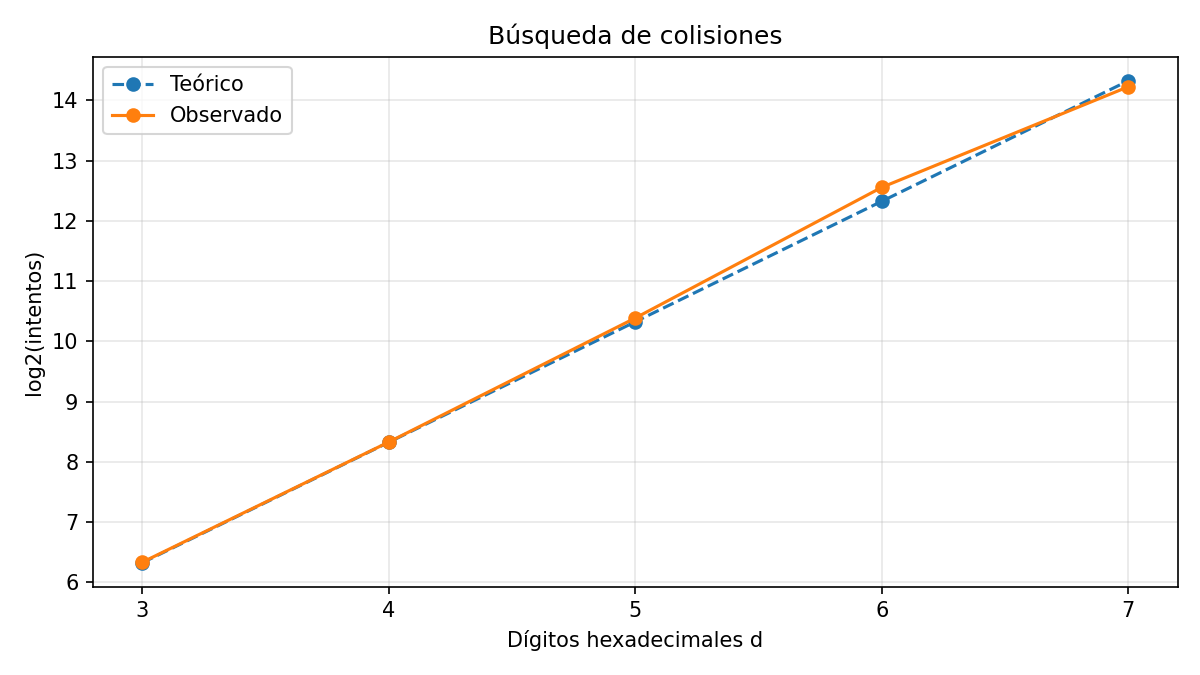
\includegraphics[width=0.9\linewidth]{../outputs/colisiones/colisiones_vs_d.png}
    \caption{Comparación entre el costo teórico y observado para la búsqueda de colisiones.}
\end{figure}

Graficamente vemos la similaridad entre los valores teóricos y los observados.
\subsection{Prueba 3: Resistencia a preimágen}
\subsection{Resistencia a preimágenes}
\begin{table}[H]
\centering
\renewcommand{\arraystretch}{1.2}
\small
\begin{tabularx}{\textwidth}{lXXXXXXX}
\toprule
$d$ (hex) & $n$ (bits) & Intentos teóricos & Intentos obs. & Mediana & Repeticiones \\
\midrule
3 & 12 & 4096 & 4211.57 & 3023.0 & 100 \\
4 & 16 & 65536 & 52958.11 & 42902.0 & 100 \\
5 & 20 & 1048576 & 877756.47 & 563780.5 & 30 \\
6 & 24 & 16777216 & 13479409.30 & 11948610.5 & 10 \\
7 & 28 & 268435456 & 429821378.33 & 218920444.0 & 3 \\
\bottomrule
\end{tabularx}
\caption{Resultados experimentales para la búsqueda de preimágenes a distintas longitudes de digest.}
\end{table}
En este caso, podemos observar que los valores teóricos se alejan para $d \in \{6,7\}$ dado que al tener cómputo limitado no fue posible correr el experimento tantas veces cómo era requerido para acercarse al valor teórico.
\begin{figure}[h]
    \centering
    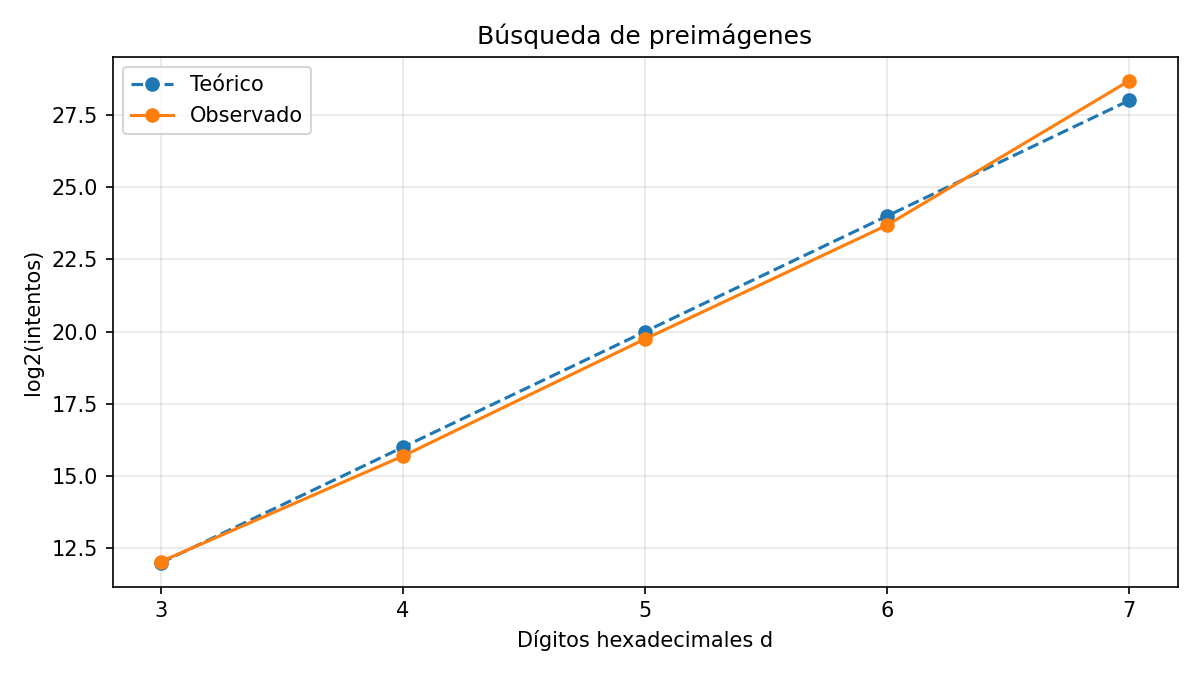
\includegraphics[width=0.9\linewidth]{../outputs/preimagen/preimagen_vs_d.png}
    \caption{Comparación entre el costo teórico y observado para la búsqueda de preimágenes.}
\end{figure}

Para verificar si nuestra función hash es correcta en su construcción, realizamos la siguiente comparación.
\begin{equation}
    \frac{T_{preimagen}(d)}{T_{colision}(d)}
\end{equation}
Con los datos reales obtenidos para $d$ = 4 tenemos:
\begin{equation}
    \frac{52,958{.}11}{321{.}76} \approx 164{.}6
\end{equation}
El valor teórico está cerca de 200. No está muy desviado nuestro valor experimental pero para confirmar si la tendencia general es correcta, calculamos para $d$ = 5.
\begin{equation}
    \frac{877,756{.}47}{1340{.}14} \approx 655
\end{equation}
La tendencia es correcta: la preimagen se vuelve mucho más costosa que la colisión conforme aumenta $d$.

\subsection{Prueba 4: Resistencia a segunda preimágen}
\begin{table}[H]
\centering
\small
\renewcommand{\arraystretch}{1.2}
\begin{tabular}{lcccccc}
\toprule
$d$ (hex) & $n$ (bits) & Intentos teóricos & Intentos obs. & Tiempo medio & Repeticiones & $\rho(d)$ \\
\midrule
3 & 12 & 4096 & 4551.21 & 314.10 ms & 100 & 1.081 \\
4 & 16 & 65536 & 60255.43 & 4102.32 ms & 100 & 1.138 \\
5 & 20 & 1048576 & 950484.13 & 85071.10 ms & 30 & 1.083 \\
6 & 24 & 16777216 & 14245918.60 & 635488.60 ms & 10 & 1.056 \\
7 & 28 & 268435456 & 211628060.67 & 7121828.17 ms & 3 & 0.492 \\
\bottomrule
\end{tabular}
\caption{Comparación experimental entre la búsqueda de segunda preimagen y la de preimagen.}
\end{table}
donde $\rho(d)$ es igual a:
\begin{equation}
    \rho(d) = \frac{T_{2^a preimagen}(d)}{T_{preimagen}(d)}
\end{equation}
Los resultados experimentales coinciden con la teoría.\\
La teoría dice que ambos ataques deberían tener el mismo costo esperado, por lo que
$\rho(d) \approx 1$. En los casos $d = 3,4,5,6$ eso ocurre bastante bien: la razón está muy cerca de 1.\\

Intentamos encontrar defectos en el diseño utilizando las siguientes pruebas que no son de fuerza bruta. 
\begin{table}[H]
\centering
\small
\renewcommand{\arraystretch}{1.2}
\begin{tabular}{p{4cm} p{5.3cm} c}
\toprule
Prueba & Qué se explota & Resultado \\
\midrule
Relleno ambiguo & $H(M) \stackrel{?}{=} H(M \| 0x00\ldots)$ si el padding no codifica la longitud original. & NO \\
Permutación de bloques & $H(m_1 \| m_2) \stackrel{?}{=} H(m_2 \| m_1)$. Si falla la conmutatividad, se rompe la estructura. & NO \\
Extensión de longitud & Dado $H(M)$, calcular $H(M \| X)$ sin conocer $M$. Debilidad clásica de Merkle-Damgård. & NO \\
Linealidad sobre $\mathbb{F}_2$ & Buscar $\Delta$ tal que $H(M \oplus \Delta) = H(M)$ para todo $M$. & NO \\
Puntos fijos & Hallar $(h,m)$ con $f(h,m)=h$ para insertar bloques sin alterar el digest. & NO \\
\bottomrule
\end{tabular}
\caption{Pruebas estructurales de segunda preimagen aplicadas al hash artesanal.}
\end{table}
Los resultados indican que no se encontraron fallas estructurales evidentes. Esto no significa que el hash sea seguro, sino que no parece presentar una debilidad estructural inmediata
\section{Discusión y conclusiones}
La comparación entre colisión, preimagen y segunda preimagen muestra una relación coherente con la teoría. La colisión resulta ser el ataque más accesible, mientras que la preimagen y la segunda preimagen requieren un costo mucho mayor. La Figura~\ref{fig:comparativa_ataques} resume esta tendencia. En ella se observa que la curva de colisión crece de manera más lenta que las curvas de preimagen y segunda preimagen, una diferencia que coincide con la expectativa teórica del modelo aleatorio. En otras palabras, el comportamiento empírico mantiene la jerarquía esperada de complejidades: la colisión es la propiedad más débil y la preimagen es la más costosa de atacar.

\begin{figure}[h]
    \centering
    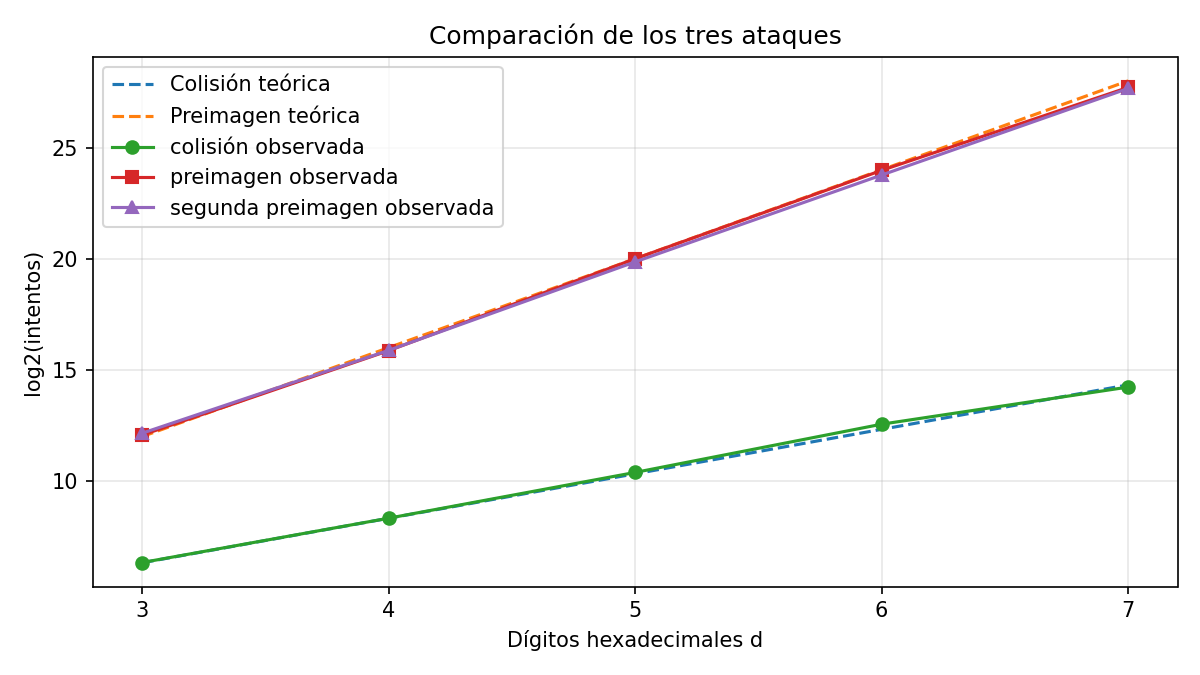
\includegraphics[width=0.9\linewidth]{../outputs/segunda_preimagen/comparativa_tres_ataques.png}
    \caption{Comparación empírica de los costos observados para colisión, preimagen y segunda preimagen.}
    \label{fig:comparativa_ataques}
\end{figure}

El cuadro 6~\ref{tab:comparativa_ataques} refleja este comportamiento de forma cuantitativa. En todos los casos evaluados, el costo observado crece exponencialmente con la longitud del digest, y la separación entre colisión y preimagen se mantiene de la misma manera que la teoría predice. Sin embargo, la diferencia entre los valores teóricos y observados en algunos puntos indica que la experimentación está influida por la variabilidad estadística y por el número limitado de repeticiones, particularmente para $d=7$.

\begin{table}[h]
\centering
\renewcommand{\arraystretch}{1.2}
\begin{tabular}{lcccc}
\toprule
Ataque & El atacante elige & Costo ideal & Pendiente en $d$ & Intentos $(d=6)$ \\
\midrule
Colisión & $M$ y $M'$ & $2^{2d}$ & 2 & $\approx 5.13 \times 10^3$ \\
Segunda preimagen & solo $M'$ & $2^n$ & 4 & $\approx 1.68 \times 10^7$ \\
Preimagen & nada & $2^n$ & 4 & $\approx 1.68 \times 10^7$ \\
\bottomrule
\end{tabular}
\caption{Comparación del costo esperado para colisión, preimagen y segunda preimagen.}
\label{tab:comparativa_ataques}
\end{table}

La evaluación de segunda preimagen estructural también es útil para establecer un marco de referencia: ninguna de las pruebas explotadas por ataque clásico fue efectiva. En particular, las pruebas de padding ambiguo, permutación de bloques, extensión de longitud, linealidad sobre $\mathbb{F}_2$ y puntos fijos no mostraron un camino real para construir una segunda preimagen sin costo significativo. Este resultado indica que el diseño no presenta una debilidad estructural evidente bajo las estrategias analizadas, aunque tampoco sugiere que pueda considerarse un algoritmo seguro para uso práctico.

En conclusión, la función propuesta funciona para entender la dinámica de una función hash y para medir propiedades fundamentales de seguridad. Los resultados experimentales muestran un comportamiento compatible con el modelo aleatorio en varias dimensiones, especialmente en el efecto avalancha y en la escala creciente del costo para colisiones y preimágenes. Sin embargo, la implementación no cumple con los estándares de seguridad de sistemas criptográficos reales.

\end{document}